
\subsection{Integral curves and flows}

For manifolds with boundary we essentially define integral curves in the same way as for boundaryless manifolds, but allow the domain to be any non-trivial interval (i.e. not a single point) containing $0$. In particular this interval may only be half-open or closed. In general, the existence of integral curves on manifolds with boundary fails as illustrated by the following example:

\begin{counterexample}
    \label{rem:vector_field_example}
    Consider  the lower halfspace $M := \R^2_{y \leq 0}$ and the vector field $X := \frac{\partial}{\partial x} + 2x \frac{\partial}{\partial y}$. Then for $p = (0,0)$ the integral curve is only defined for $t = 0$, since on $\R^2$ it would be given by $\gamma(t) = (t,t^2)$ but $t^2 > 0$ for $t \neq 0$.
    \begin{figure}[ht]
        \centering
        \label{fig:vector_field1}
        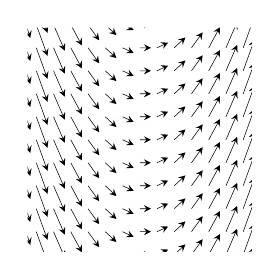
\begin{tikzpicture}[scale = 0.5,every plot/.append style={very thick}]
    \begin{axis}[
        clip = true,
        ticks = none,
        xmin = -1.5, xmax = 1.5,
        ymin = -1.5, ymax = 1.5,
        zmin = 0, zmax = 1,
        axis equal image,
        axis lines = middle,
        axis line style={draw=none},
        view = {0}{90},
    ]
        \addplot3[samples = 27,
            quiver = {
                u = {1},
                v = {2*x},
                scale arrows = 0.15,
            },
            -stealth,
            domain = -3:3,
            domain y = -4:4,
        ] {0};
    \end{axis}
    
\end{tikzpicture}
        \caption{The vector field $X$. The integral curves are parabolas.}
    \end{figure}
\end{counterexample}

We do however still get a uniqueness result \textit{if} the integral curve exists. Furthermore, if the vector field is sufficiently well-behaved we can guarantee the existence.

\begin{theorem}[Uniqueness and existence of Integral curves]
    \label{lem:existence_integral_curves}
    Let $M$ be a manifold with boundary, $X$ a smooth vector field on $M$ and $p \in M$. If there exists an integral curve starting at $p$, then there exists a unique maximal integral curve $\gamma \colon I \to M$ starting at $p$, where one of the four following cases holds for $a \leq 0 \leq b$, $a<b$:
    \begin{enumerate}[(i)]
        \item $I = (a,b)$
        \item $I = [a,b)$ and $\gamma(a) \in \partial M$
        \item $I = (a,b]$ and $\gamma(b) \in \partial M$
        \item $I = [a,b]$ and $\gamma(a),\gamma(b) \in \partial M$
    \end{enumerate}
    Furthermore, if $X$ is either transversal to the boundary or everywhere tangent, the unique maximal integral curve starting at $p$ always exists.
\end{theorem}

\begin{proof}Let's begin by showing uniqueness. The proof is essentially the same as in the boundaryless case (see for example \cite{lee2011smooth}): We show that two integral curves $\gamma \colon I \to M$ and $\gamma^\prime \colon I^\prime \to M$ starting at $p$ agree on their common domain. This then allows us to define the maximal integral curve on some interval $I$ and every interval containing $0$ is of the form $(i) - (iv)$ \footnotemark. The only difference is that $I$ and $I^\prime$ may not be open intervalls. So we have to show that uniqueness still applies. We claim: Let $U \subseteq \R^n$ be open, $F \colon U \to \R^n$ a smooth vector field, $I$ an interval of the form $(i) - (iv)$ and $\gamma,\gamma^\prime \colon I \to U$ integral curves both starting at $p \in U$. Then $\gamma = \gamma^\prime$. If $0$ is an interior point of $I$ we can apply the usual uniqueness theorem for $\gamma,\gamma^\prime$ restricted to $\mathrm{int}(I)$. By continuity they must then also agree at the endpoint. So it remains to show uniqueness if $0$ is a boundary point of $I$ (say for example $I = [0,b)$). But by the existence theorem for integral curves we can find an integral curve $\eta \colon (-\epsilon,\epsilon) \to U$ starting at $p$ and define
\[
\beta \colon (-\epsilon,b) \to U, t \mapsto \begin{dcases*}
    \eta(t), t \leq 0 \\
    \gamma(t), t \geq 0
\end{dcases*}
\]
Since $\eta(0) = \gamma(0)$ and $\dot{\eta}(0) = F(p) = \dot{\gamma}(0)$ we get that $\beta$ is at least $C^1$. Similiarly we define
\[
\beta^\prime \colon (-\epsilon,b) \to U, t \mapsto \begin{dcases*}
    \eta(t), t \leq 0 \\
    \gamma^\prime(t), t \geq 0
\end{dcases*}
\]
By the uniqueness theorem we have
\[
\beta = \beta^\prime
\]
and our claim follows. The case $I = (a,0]$ goes analogous and for $I = [0,b]$ or $I = [a,0]$ it is either trivial (if $a = b = 0$) or we consider $I\setminus \{b\}$ resp. $I\setminus \{a\}$ and apply the above argument. Equality at $t = a, t = b$ respectively then again follows by continuity.

To see that $\gamma(t) \in \partial M$ for $t \in \{a,b\}$ a boundary point of $I$ we note that for $ p = \gamma(t) \in \mathrm{int}(M)$ we can define the integral curve starting at $p$ on some open interval $(-\epsilon,\epsilon)$ by the existence theorem for integral curves (Picard-Lindelöff). But then $t$ is not a boundary point of $I$ since $I$ is maximal.

Next we show the existence if $X$ is transversal to $\partial M$. For $p \in \mathrm{int}(M)$ this follows directly from the Picard-Lindelöff Theorem as in the boundaryless case. If $p \in \partial M$, we may argue similiarly: Consider a chart $h \colon \R^n_{x_n \geq 0} \supseteq U \to M$ around $p = h(0)$ and let $Y$ be the vector field $X$ in this chart, i.e. $D_q h(Y_q) = X_{h(q)}$. Then by definition of smoothness we can extend $Y$ to a smooth vector field $Y^\prime$ on some open neighbourhood $U^\prime \subseteq \R^n$ around $0 = h^{-1}(p)$. Applying Picard-Lindelöff we get the existence of an integral curve $\gamma \colon (-\epsilon,\epsilon) \to U^\prime$ of $Y^\prime$ starting at $0$. Write $$Y^\prime = \sum_i F_i \frac{\partial}{\partial x_i}$$ and $$\gamma = (\gamma_1,\ldots,\gamma_n).$$ Assume that $X$ is inwards pointing along the boundary. After restricting to a smaller domain we may assume $F_n \geq 0$. Then
\[
\gamma^\prime_n(t) = F_n(\gamma(t)) \geq 0,
\]
such that $\gamma_n$ is increasing. In particular $\gamma_n(t) \geq 0$ for $t \in [0,\epsilon)$, hence $\gamma(t) \in U$ for $t \in [0,\epsilon)$. Then $$\eta := h \circ \gamma \colon [0,\epsilon) \to M$$ is the desired integral curve.

For the case that $X$ is everywhere tangent to $\partial M$ see \cite{lee2011smooth} (Theorem 9.34).
    
\end{proof}

\footnotetext{If we put together integral curves defined on open intervals that agree on their common domain, it is clear that this results in a smooth curve, since around each $t$ this curve is given by one of the smooth curves which we put together. If we put together integral curves $\gamma_1,\gamma_2$ defined on something like $I_1 = (a,b]$ and $I_2 = [b,c)$ we have to be more careful around the boundary point $b$. But the same argument as we applied to $\beta$ in the proof of Lemma \ref{lem:existence_integral_curves} shows that putting $\gamma_1$ and $\gamma_2$ together results in a $C^1$-curve. We can then apply the usual uniqueness theorem to see that this curve is already given by a $C^\infty$-curve.}

On compact manifolds we can say more about the maximal Interval $I$:
\begin{lemma}[Existence of Integral curves on compact manifolds]
\label{lem:existence_integral_curves_compact_mnf}
    If $M$ is compact in Lemma \ref{lem:existence_integral_curves} then the maximal interval $I$ has one of the following forms:
    \begin{enumerate}[(i)]
        \item $I = (-\infty,\infty)$
        \item $I = [a,\infty)$ and $\gamma(a) \in \partial M$
        \item $I = (-\infty,b]$ and $\gamma(b) \in \partial M$
        \item $I = [a,b]$ and $\gamma(a),\gamma(b) \in \partial M$
    \end{enumerate}
\end{lemma}
\begin{proof}
Let $\gamma \colon I \to M$ be the unique maximal integral curve guaranteed by Lemma \ref{lem:existence_integral_curves}. We will show that any open boundary point of $I$ must be $\pm \infty$. For simplicity let us only consider $I = [a,b)$. The other cases are completely analogous. By compactness we can find a sequence $0 < t_n \nearrow b$ such that $\gamma(t_n)$ coverges to a point $q \in M$.

\noindent \textbf{Case 1: $q \in \mathrm{int}(M)$.} By Picard-Lindelöff we can find an open neighbourhood $U \subseteq M$ around $q$ and $\epsilon > 0$, such that for every point $x \in U$ the intgeral curve starting at $x$ is defined for $t \in (-\epsilon,\epsilon)$. For some fixed $m$ sufficiently large we have $q_0 := \gamma(t_m) \in U$. Assume that $b - t_m < \frac{\epsilon}{2}$. But then we can extend $\gamma$ to $[a,b + \frac{\epsilon}{2})$ as follows. Consider
\[
\gamma^\prime \colon [a-t_m,b-t_m) \to M, \; t \mapsto \gamma(t + t_m).
\]
Then $\gamma^\prime$ is a integral curve starting at $q_0$. Let $\alpha \colon (-\epsilon,\epsilon) \to M$ be another integral curve starting at $q_0$. Then $\alpha$ and $\gamma^\prime$ agree on their common domain by the arguments in Lemma $\ref{lem:existence_integral_curves}$ and thus we can put them together to define an integral curve 
\[
\beta \colon J \to M
\]
for $J := [a-t_m,b-t_m) \cup (-\epsilon,\epsilon) \supseteq [a-t_m,\epsilon)$. But then we can define
\[
\gamma^{\prime\prime} \colon [a,\epsilon + t_m) \to M, \; t \mapsto \beta(t-t_m),
\]
which is an integral curve starting at $\gamma(0) = p$. However
\[
b + \frac{\epsilon}{2} < t_m + \epsilon
\]
and so $[a,b + \frac{\epsilon}{2}) \subseteq [a,\epsilon + t_m)$, contradicting maximality of $\gamma$.

\noindent \textbf{Case 2: $q \in \partial M$.} We argue similiarly as above. In a local chart around $q$ we can again apply Picard-Lindelöff (smoothness of $X$ guarantees by definition the existence of a smooth extension of $X$ to an open neighbourhood in $\R^n$). We then again take $q_0 := \gamma(t_m)$ sufficiently close to $q$, choose an integral curve $\alpha$ starting at $q$, which we can use to define an integral curve $\alpha^\prime$ starting at $q_0$ defined on some open interval $(-\epsilon,\epsilon) $ by translation in time as above. Also we define $\gamma^\prime$ as above. The same argument as above then shows that we can extend $\gamma^\prime$ (in the local chart) to an integral curve $\beta$ on $J := [a-t_m,b-t_m) \cup (-\epsilon,\epsilon) \supseteq [a-t_m,b-t_m]$. In particular we have $\beta([a-t_m,b-t_m]) \subseteq M$. Translating in time again yields an integral curve $\gamma^{\prime\prime} \colon [a,b] \to M$ contradicting maximality.
\end{proof}

As an application we can show:

\begin{lemma}
    Let $I$ be some proper interval containing $0$ and $\gamma \colon I \to M$ any smooth regular curve, i.e. $\dot{\gamma}(t) \neq 0$ for all $t \in I$. Then there exists a unique unit speed reparametrization of $\gamma$, that is an orientation preserving diffeomorphism $\phi \colon J \to I$ with $\phi(0) = 0$, such that $\gamma \circ \phi$ is a unit speed curve. 
\end{lemma}

\begin{proof}
    We have 
    \[
    (\gamma \circ \phi)^{\raisebox{2pt}{\scalebox{0.4}{$\bullet$}}}(t) = \phi^\prime(t) \dot{\gamma}(\phi(t)),
    \]
    so we need to find $\phi$, such that (note that we also need $\phi^\prime > 0$ to preserve orientation)
    \[
    \phi^\prime(t) = \frac{1}{\abs{\dot{\gamma}(\phi(t))}}
    \]
    This is a flow equation for the smooth vector field
    \[
    X(p) := \frac{1}{\abs{\dot{\gamma}(p)}}
    \]
    on $I$. Since $X$ is transversal to the boundary of $I$ (if $I$ even has boundary), Theorem \ref{lem:existence_integral_curves} yields the existence of a unique maximal integral curve $\phi \colon J \to I$ of $X$ with $\phi(0) = 0$. We now only need to show that $\phi$ is surjective, since $\phi^\prime >0$ already shows that it is an embedding. 
    
    To this end, consider any compact subinterval $I^\prime := [a,b] \subseteq I$ ($a < b$) containing $0$ and let $\psi \colon J^\prime \to I^\prime$ be the unique maximal integral curve of $X|_{I^\prime}$ starting at $0$. By Lemma \ref{lem:existence_integral_curves_compact_mnf} $\psi$ has to be defined on a compact interval $J^\prime = [c,d]$, since $X|_{I^\prime}$ is bounded below by a positive constant, so if $J^\prime$ would be infinite in the positive/negative direction, $\psi$ would also tend to positive/negative ininity, but by definition it is conatined in the compact interval $I^\prime$. Moreover Lemma \ref{lem:existence_integral_curves_compact_mnf} then yields
    \[
    \psi(c) = a, \quad \psi(d) = b.
    \]
    Since $\phi$ is the unique maximal integral curve of $X$ we get that $J^\prime \subseteq J$ and $\phi|_{J^\prime} = \psi$. In particular $I^\prime \subseteq \mathrm{im}(\phi)$. This completes the proof.
\end{proof}

\begin{remark}[A note on flows for manifolds with boundary]
    In general the concept of a flow is not well behaved if $M$ has boundary, as integral curves may not even exist (see Counterexample \ref{rem:vector_field_example}). In \cite{lee2011smooth} the author shows, that if $X$ is tangent to $\partial M$ we still get a well-behaved flow, i.e. it is defined on some open subset $\mathcal{O} \subseteq M \times \R$. I think that if we instead assume, that $X$ is transversal to $\partial M$, we still get a "good" flow domain in the sense that we can define the flow on some subset $\mathcal{D} \subseteq M \times \R$, which is a codimension $0$ submanifold with boundary and $I_p := \{ t \in \R \mid (p,t) \in \mathcal{D}\}$ is an interval around $0$ for each $p \in M$.
\end{remark}

The statement in the above remark should follow from the following lemma, which allows us to define submanifold charts for $\mathcal{D}$.

\begin{lemma}
    Let $M$ be a manifold with boundary and $X$ a vector field of $M$, which is inward pointing along $\partial M$. Let 
    \[
    M_{\partial} := \{p \in M \mid \mathrm{im}\gamma_p \cap \partial M \neq \emptyset\}
    \]
    be all points in $M$ whose trajectory contains boundary points (this is at most one for each $p \in M$). For $p \in M_\partial$ the integral curve $\gamma_p$ starting at $p$ is defined on some interval $[-\tau(p),a)$ for some $\tau(p) \geq 0$ and $a > -\tau(p)$. Then the following statements hold true
    \begin{enumerate}[(i)]
        \item $M_\partial$ is an open subset of $M$
        \item $\tau \colon M_\partial \to \R_{\geq 0}, \, p \mapsto \tau(p)$ is smooth
    \end{enumerate}
\end{lemma}
\begin{proof}[Proof sketch]
    The idea is to consider the maximal flow
    \[
    \theta \colon \mathcal{D} \to M, \; (p,t) \mapsto \gamma_p(t)
    \]
    on some open subset $\mathcal{D} \subseteq \partial M \times [0,\infty)$ and show that this is an embedding. Then 
    \[
    M_\partial = \mathrm{im} \theta
    \]
    is open and 
    \[
    \tau = \pi \circ \theta^{-1} \colon M_\partial \to [0,\infty)
    \]
    where $\pi \colon \partial M \times [0,\infty) \to [0,\infty)$ is the canonical projection map.
\end{proof}


% \begin{lemma}
%     \LARGE \textcolor{red}{Injective Flowouts are already embeddings}
% \end{lemma}